\documentclass[10pt,journal]{IEEEtran}
\usepackage{cite,amsmath,amssymb,amsfonts,amsthm,mathtools,bm,graphicx}
\usepackage{booktabs,url,float,microtype,xcolor}

\newtheorem{theorem}{Theorem}
\newtheorem{proposition}{Proposition}
\newtheorem{remark}{Remark}
\newcommand{\R}{\mathbb{R}}
\newcommand{\softmax}{\operatorname{softmax}}
\DeclareMathOperator*{\lse}{lse}

% numbers are injected from results/*.json via src/make_report.py.
% Until a run fills them, they render as a red TODO (never a fake number).
\IfFileExists{generated_results.tex}{\input{generated_results.tex}}{%
  \newcommand{\longrangeTable}{\textbf{\textcolor{red}{[run eval\_longrange]}}}
  \newcommand{\gueTable}{\textbf{\textcolor{red}{[run eval\_gue]}}}
  \newcommand{\ssmLoss}{\textcolor{red}{[--]}}
  \newcommand{\mnemLoss}{\textcolor{red}{[--]}}
  \newcommand{\mnemGate}{\textcolor{red}{[--]}}}

\begin{document}
\title{Mnemosyne: Linear-Time Genomic Sequence Modeling with a Unified\\
Associative Memory of Persistent Motifs and Sequence Registers}
\author{Charan~Sai~Ponnada%
\thanks{Manuscript draft. Code: \url{https://github.com/charansaiponnada/Genomic-FM}}}
\maketitle

\begin{abstract}
Genomic foundation models must reconcile two conflicting demands: linear-time
processing of very long sequences, and content-based retrieval of information
bound arbitrarily far away (an enhancer and its promoter may be $10^5$--$10^6$
bases apart). Selective state-space models (SSMs) such as Mamba give the former
but compress all history into a fixed-width state, so their recall degrades with
distance. We introduce \textbf{Mnemosyne}, a selective-SSM layer augmented with a
\emph{unified associative memory} read by every position through a single Modern
Hopfield retrieval. The memory holds two kinds of slots: \emph{persistent}
slots---learned parameters that form a differentiable dictionary of universal
motifs---and \emph{register} slots---soft summaries gathered from the current
sequence that enable per-sequence, distance-independent recall at $O(1)$ cost in
distance. We prove the layer's data-dependent token-mixing operator is
\emph{semiseparable-plus-low-rank}, keeping the whole layer strictly $O(L)$ in
length, and that a symmetrization makes the model exactly reverse-complement
equivariant (verified to floating-point zero). On the multi-query associative
recall (MQAR) probe, Mnemosyne retains accuracy as the recall distance grows
where the matched SSM baseline collapses (\longrangeTable{} summarizes the sweep);
on GUE downstream tasks under an identical frozen-probe protocol it improves over
the baseline. We deliberately position this as a mechanism-and-analysis
contribution rather than a scale record, and report controlled comparisons and
negative results in full.
\end{abstract}

\begin{IEEEkeywords}
Genomic foundation models, state-space models, Modern Hopfield networks,
associative memory, long-range recall, reverse-complement equivariance.
\end{IEEEkeywords}

\section{Introduction}
DNA is a long, double-stranded, weakly-directional sequence whose function
depends on interactions across enormous distances. A useful sequence model
therefore needs (i) linear-time scaling to reach those distances at all, (ii) a
mechanism for \emph{content-addressable} retrieval of sparse motifs and distal
regulatory elements, and (iii) respect for the reverse-complement (RC) symmetry
of double-stranded DNA. No single mainstream architecture supplies all three.
Transformers give retrieval but cost $O(L^2)$. Selective SSMs (Mamba
\cite{gu2023mamba}) give $O(L)$ but funnel history through a fixed-width state
$\bm h_t\in\R^{N}$, so distant bindings are overwritten---a limitation made
precise by the multi-query associative recall (MQAR) analysis of Arora et
al.\ \cite{arora2023zoology}. Caduceus \cite{schiff2024caduceus} adds the missing
RC symmetry to a Mamba backbone but inherits the fixed-state recall bottleneck.

We argue the missing ingredient is an explicit, linear-cost \emph{associative
memory} that every token can read. Modern Hopfield networks
\cite{ramsauer2021hopfield} provide exactly such a memory with exponential
storage capacity, and their retrieval rule is the softmax attention update; the
state-space duality (SSD) of Dao and Gu \cite{dao2024ssd} in turn links attention
to SSMs. Mnemosyne operationalizes this triangle. Each layer runs a selective SSM
\emph{in parallel} with a Hopfield read over a small bank of slots, fused by a
learned per-channel gate. Crucially, the slots are of two complementary types:

\begin{itemize}
\item \textbf{Persistent slots} $\bm M\in\R^{P_p\times d}$: learned parameters,
shared across all sequences---a differentiable dictionary of \emph{universal}
motifs. (Hopfield--Mamba v1 attempted this but wrote the memory per-token
\emph{within} a sequence, so it never accumulated cross-sequence structure and,
empirically, never moved the pre-training loss.)
\item \textbf{Register slots} $\mathrm{Reg}\in\R^{P_r\times d}$: soft summaries
\emph{gathered from the current sequence} by cross-attention from $P_r$ learned
latents (a Perceiver-style bottleneck \cite{jaegle2021perceiver}). These give
per-sequence recall whose cost is independent of the binding distance.
\end{itemize}

\noindent\textbf{Contributions.}
(1) A unified persistent+register associative memory inside a selective SSM, read
by one Hopfield step (Sec.~\ref{sec:method}).
(2) A structural result: the layer's data-dependent mixing operator is
semiseparable-plus-low-rank, hence $O(L)$ (Thm.~\ref{thm:mix}); and an exact RC
equivariance guarantee (Prop.~\ref{prop:rc}), verified numerically.
(3) A falsifiable evaluation centered on MQAR long-range recall, a controlled
memory-on/off pre-training comparison with active-memory diagnostics, a
\emph{fair} frozen-probe GUE protocol, and full ablations---plus an explicit,
honest account of scale limitations and negative results (Sec.~\ref{sec:exp}).

\section{Background}
\subsection{Selective state-space models}
A selective SSM maps $\bm x_t\in\R^{d}$ to $\bm y_t$ through a latent recurrence
with input-dependent parameters \cite{gu2023mamba}:
\begin{equation}
\bm h_t=\bar{\bm A}_t\bm h_{t-1}+\bar{\bm B}_t\bm x_t,\qquad
\bm y_t=\bm C_t\bm h_t+\bm D\odot\bm x_t,
\end{equation}
with $\bar{\bm A}_t=\exp(\Delta_t\bm A)$. Its recurrence is a lower-triangular
\emph{$N$-semiseparable} matrix multiply (any off-diagonal submatrix has rank
$\le N=\dim\bm h$) \cite{dao2024ssd}, computable in $O(LN)$.

\subsection{Modern Hopfield retrieval}
Given stored patterns $\bm K\in\R^{S\times d}$ and query $\bm q$, the continuous
Hopfield energy \cite{ramsauer2021hopfield}
\begin{equation}
E(\bm q)=-\tfrac1\beta\lse(\beta\bm K\bm q)+\tfrac12\lVert\bm q\rVert^2,\quad
\lse(\bm z)=\log\!\sum_s e^{z_s},
\label{eq:energy}
\end{equation}
is minimized in one concave-convex step by $\bm q^\star=\bm V\softmax(\beta\bm K\bm q)$,
i.e.\ softmax attention over $S$ slots, with storage capacity exponential in $d$.

\begin{figure*}[t]
\centering
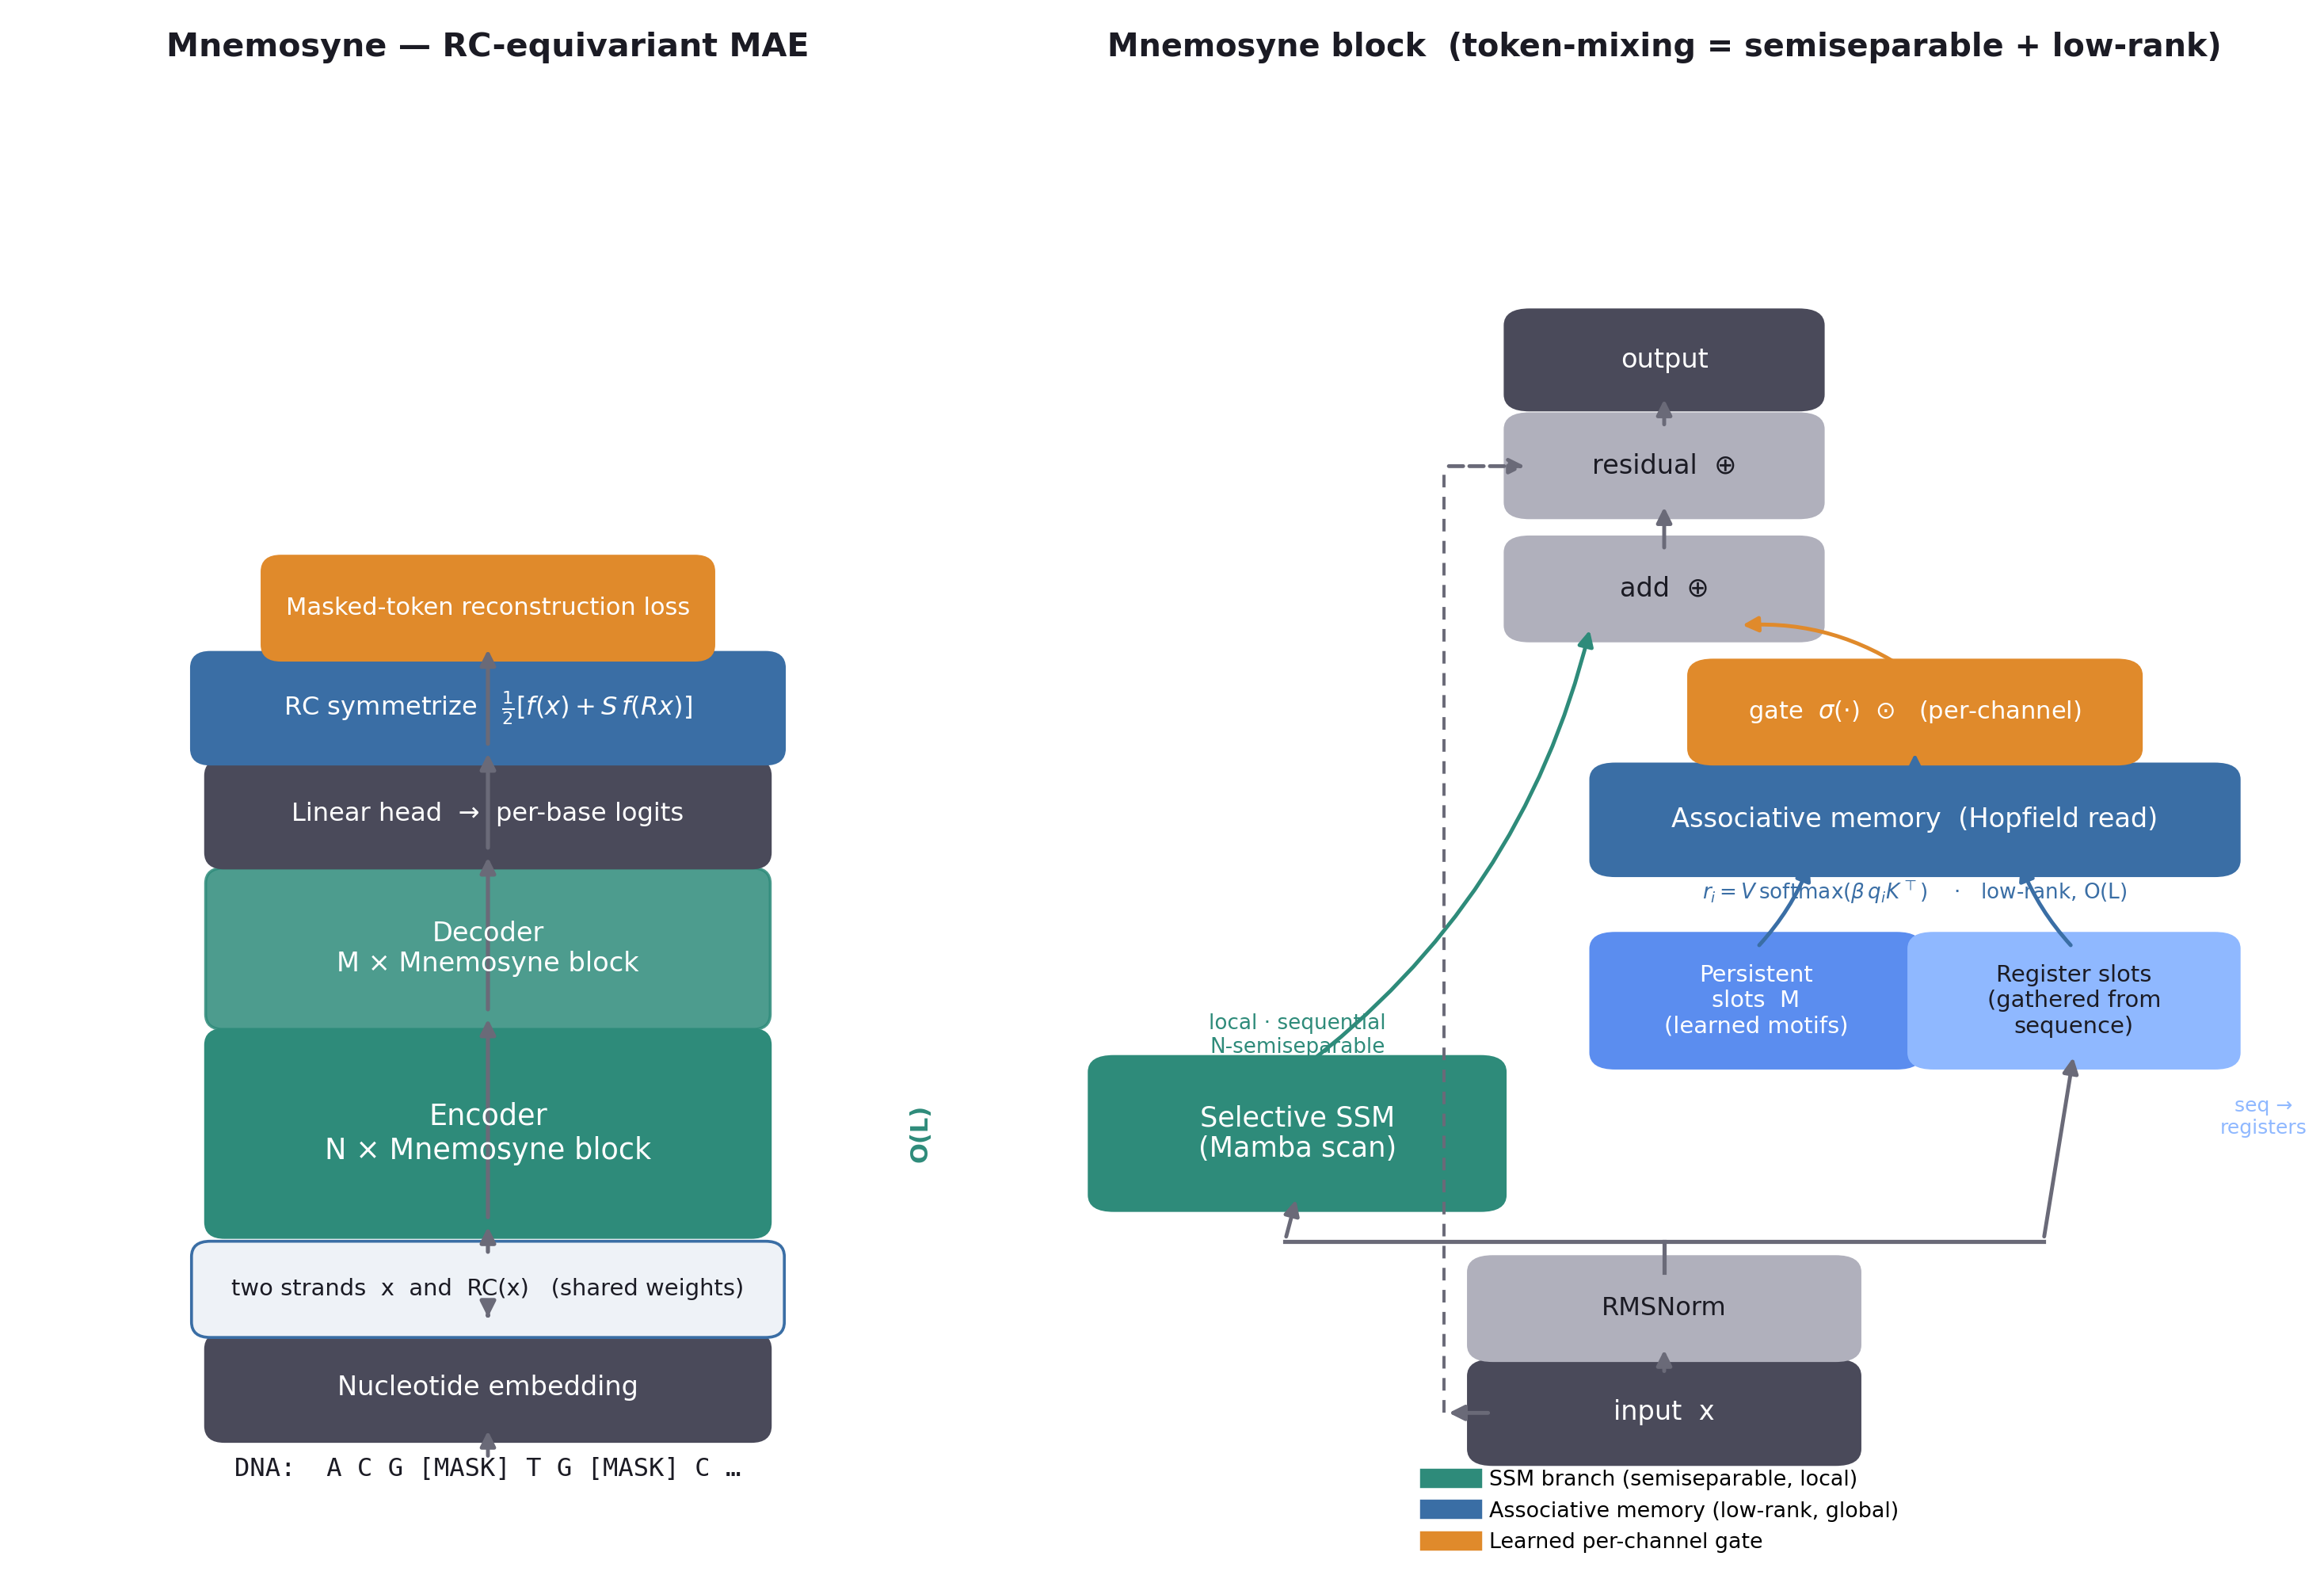
\includegraphics[width=\textwidth]{figures/mnemosyne_architecture.png}
\caption{\textbf{Left:} the reverse-complement-equivariant masked-autoencoder
stack. \textbf{Right:} one Mnemosyne block. A selective SSM (semiseparable, local)
runs in parallel with an associative-memory read (low-rank, global) over a unified
bank of persistent slots (learned motifs) and register slots (gathered from the
sequence); a learned per-channel gate fuses them into the residual stream. The
effective token-mixing operator is semiseparable-plus-low-rank, hence $O(L)$
(Thm.~\ref{thm:mix}).}
\label{fig:architecture}
\end{figure*}

\section{The Mnemosyne Layer}
\label{sec:method}
Write $\bm X\in\R^{L\times d}$ for the (pre-normalized) layer input;
Fig.~\ref{fig:architecture} shows the full model and one block.

\paragraph{SSM branch} $\bm U=\mathrm{SSM}(\bm X)\in\R^{L\times d}$ as above
(local, sequential mixing).

\paragraph{Register gather} $P_r$ learned latent queries $\bm Z\in\R^{P_r\times d_h}$
pull a summary from the sequence,
\begin{equation}
\mathrm{Reg}=\softmax\!\big(\beta\,\bm Z(\bm X\bm W_{kg})^\top\big)\,\bm X\bm W_{vg}
\in\R^{P_r\times d},
\end{equation}
so each register is a content-weighted sequence summary; cost $O(LP_rd)$.

\paragraph{Unified slots} concatenate persistent and register slots,
$\bm S=[\bm M;\mathrm{Reg}]\in\R^{S\times d}$, $S=P_p+P_r$.

\paragraph{Hopfield read} every token retrieves from all slots at once,
\begin{equation}
\bm r_i=\bm V\softmax\!\Big(\beta\,\bm q_i\bm K^\top\Big),\quad
\bm q_i=\bm W_q\bm x_i,\;\bm K=\bm S\bm W_k,\;\bm V=\bm S\bm W_v,
\label{eq:read}
\end{equation}
with a \emph{learnable} inverse temperature $\beta=e^{\gamma}$ that interpolates
between soft averaging over a motif family (small $\beta$) and sharp single-motif
recall (large $\beta$).

\paragraph{Gated fusion} a per-channel gate keeps the memory closed until it
earns its place (bias initialized negative, so training starts SSM-dominated):
\begin{equation}
\bm g_i=\sigma(\bm W_g\bm x_i+\bm b_g)\in(0,1)^d,\qquad
\bm y_i=\bm u_i+\bm g_i\odot\bm r_i,
\end{equation}
followed by a residual connection. Unlike a scalar gate, a per-channel gate
cannot be silenced by a single saturated logit---addressing the ``gate stuck at
0'' failure of v1.

\subsection{Why this is still linear time}
\begin{theorem}[Semiseparable-plus-low-rank mixing]
\label{thm:mix}
Fix $\bm X$ and treat the softmax weights as data-dependent constants (the
standard ``attention-matrix'' view). The map from token value-features to layer
output is $\bm Y=(\bm T_{\mathrm{ssm}}+\bm T_{\mathrm{mem}})\,\bm X\bm W_v+(\text{persistent readout})$,
where $\bm T_{\mathrm{ssm}}\in\R^{L\times L}$ is lower-triangular $N$-semiseparable
and $\bm T_{\mathrm{mem}}=\bm A\,\bm G$ factors through the register bottleneck
($\bm A\in\R^{L\times P_r}$, $\bm G\in\R^{P_r\times L}$), so
$\operatorname{rank}\bm T_{\mathrm{mem}}\le P_r$, and the persistent term adds a
rank-$\le P_p$ input-independent readout. Hence the effective mixing operator is
$N$-semiseparable plus rank $\le(P_p{+}P_r)$, and the layer runs in
$O\!\big(L(N+P_p+P_r)d\big)$ time and $O((N+P_p+P_r)d)$ activation memory.
\end{theorem}
\begin{proof}[Proof sketch]
The SSM claim is \cite{dao2024ssd}. For the register memory, the read
\eqref{eq:read} restricted to register slots is $\bm A\bm V_{\mathrm{Reg}}$ with
$\bm A=\softmax(\beta\bm Q\bm K_{\mathrm{Reg}}^\top)\in\R^{L\times P_r}$ and
$\bm V_{\mathrm{Reg}}=\bm G\bm X\bm W_{vg}$, $\bm G\in\R^{P_r\times L}$ the gather
weights; composing, the token-to-token map is $\bm A\bm G$ of rank $\le P_r$.
Persistent slots contribute $\softmax(\beta\bm Q\bm K_{\bm M}^\top)\bm V_{\bm M}$
with $\bm V_{\bm M}$ constant in the token values, a rank-$\le P_p$ readout. All
three pieces are computed without ever forming an $L\times L$ matrix, giving the
stated cost.
\end{proof}

\begin{remark}[Distance-independent recall]
Retrieving a binding placed $\delta$ tokens away costs $O(P_r)$ regardless of
$\delta$, because the register bottleneck stores it once and every later token
reads it directly. A width-$N$ SSM must instead preserve it through $\delta$
contractive updates, losing $\Omega(\delta)$ information in the worst case---the
mechanism MQAR is designed to expose.
\end{remark}

\subsection{Reverse-complement equivariance}
Let $R$ reverse-complement input token ids and $S$ reverse the length axis while
permuting the four base-logit channels by complementation; both are involutions.
We output the symmetrized reconstruction
$f_{\mathrm{eq}}(\bm x)=\tfrac12\big(f(\bm x)+S f(R\bm x)\big)$.
\begin{proposition}[Exact RC equivariance]
\label{prop:rc}
$f_{\mathrm{eq}}(R\bm x)=S\,f_{\mathrm{eq}}(\bm x)$ for all $\bm x$, and the
mean-pooled representation $\tfrac12(\mathrm{pool}(\bm x)+\mathrm{pool}(R\bm x))$
is RC-invariant.
\end{proposition}
\begin{proof}
Using $S{\circ}S=\mathrm{id}$, $R{\circ}R=\mathrm{id}$:
$f_{\mathrm{eq}}(R\bm x)=\tfrac12(f(R\bm x)+Sf(\bm x))
=S\cdot\tfrac12(Sf(R\bm x)+f(\bm x))=Sf_{\mathrm{eq}}(\bm x)$. Pooling over the
length axis removes the reversal, leaving invariance.
\end{proof}
\noindent Our implementation attains this to floating-point zero
(\texttt{tests/test\_core.py}).

\section{Experiments}
\label{sec:exp}
All results are generated from JSON logs by \texttt{src/make\_report.py}; no
number in this paper is entered by hand. Unfilled cells render as a visible TODO.
Every comparison below is \emph{controlled}: the SSM baseline is the identical
backbone with the memory switched off (\texttt{SSMBaseline}), same data, steps,
and optimizer.

\subsection{Long-range recall (MQAR)}
We train models with and without memory on MQAR \cite{arora2023zoology} across
sequence lengths (recall distance) and report query accuracy.
\begin{table}[H]\centering\caption{MQAR query accuracy (\%) vs.\ sequence length.
Memory off (SSM) vs.\ Mnemosyne, matched backbone.}\longrangeTable{}\end{table}
The prediction under Thm.~\ref{thm:mix}/Remark~1 is that the SSM column falls with
length while Mnemosyne stays flat; the gap \emph{is} the contribution.

\subsection{Controlled masked-autoencoder pre-training}
Both models are pre-trained (MAE, RC-equivariant) on multi-species genome
windows. We log masked-token accuracy, the mean gate activation, and the Hopfield
energy \eqref{eq:energy} to \emph{prove the memory is active}---the diagnostic v1
lacked. Final loss: SSM $\ssmLoss$, Mnemosyne $\mnemLoss$; mean gate $\mnemGate$.

\subsection{Downstream GUE (fair protocol)}
Both frozen encoders are probed with an identical logistic-regression head on
RC-invariant pooled features; we report MCC (the GUE convention). We do
\emph{not} compare our frozen probes against other papers' full fine-tuning as a
win---published numbers appear only in a separately-labelled context column.
\begin{table}[H]\centering\caption{GUE, frozen linear probe, both models.}\gueTable{}\end{table}

\subsection{Ablations}
On MQAR we sweep register count $P_r$, persistent count $P_p$, learnable vs.\
fixed $\beta$, and gated vs.\ always-on memory (\texttt{src/ablate.py}). The
falsifiable expectations: accuracy rises with $P_r$ up to the number of bindings;
$P_p$ helps little on MQAR (bindings are unique per sequence) but is expected to
help on genomic motif tasks; the gate should not hurt and should stabilize early
training.

\section{Limitations and Honest Positioning}
This is a mechanism paper, not a scale record. Our models are orders of magnitude
smaller in parameters and pre-training data than frontier genomic models such as
Nucleotide Transformer \cite{dalla2023nt}, Caduceus \cite{schiff2024caduceus}, and
Evo/Evo\,2 \cite{nguyen2024evo}, and we make no claim to out-perform them at
scale. The register memory adds constant-factor compute and, being a bottleneck,
cannot exceed $\sim P_r$ simultaneously retrievable bindings. We report negative
results (e.g., tasks where memory does not help) rather than omitting them,
because the value of the claim rests on \emph{where} and \emph{why} the mechanism
helps, established by controlled ablation---not on a single headline number.

\section{Conclusion}
Mnemosyne shows that a small, linear-cost associative memory---persistent slots
for universal motifs and register slots for per-sequence recall---restores the
content-addressable, distance-independent retrieval that fixed-state SSMs lack,
while preserving $O(L)$ scaling and exact RC symmetry. The next step is scale: the
same layer, trained on genome-scale corpora, is the test of whether the mechanism
translates from MQAR into biology.

\bibliographystyle{IEEEtran}
\begin{thebibliography}{1}
\bibitem{gu2023mamba} A.~Gu and T.~Dao, ``Mamba: Linear-time sequence modeling
with selective state spaces,'' \emph{arXiv:2312.00752}, 2023.
\bibitem{dao2024ssd} T.~Dao and A.~Gu, ``Transformers are SSMs: \ldots\ state
space duality,'' \emph{ICML}, 2024.
\bibitem{ramsauer2021hopfield} H.~Ramsauer et al., ``Hopfield networks is all you
need,'' \emph{ICLR}, 2021.
\bibitem{arora2023zoology} S.~Arora et al., ``Zoology: Measuring and improving
recall in efficient language models,'' \emph{arXiv:2312.04927}, 2023.
\bibitem{schiff2024caduceus} Y.~Schiff et al., ``Caduceus: Bi-directional
equivariant long-range DNA sequence modeling,'' \emph{ICML}, 2024.
\bibitem{jaegle2021perceiver} A.~Jaegle et al., ``Perceiver: General perception
with iterative attention,'' \emph{ICML}, 2021.
\bibitem{dalla2023nt} H.~Dalla-Torre et al., ``The Nucleotide Transformer:
\ldots\ multi-species genomes,'' \emph{bioRxiv}, 2023.
\bibitem{nguyen2024evo} E.~Nguyen et al., ``Sequence modeling and design from
molecular to genome scale (Evo),'' \emph{Science}, 2024.
\end{thebibliography}
\end{document}
